\section{Works Done}
\label{sec:worksDone}
\subsection{Power calculations and battery selection}


We will use raspberry pi zero wh as microcontroller and its recommended power supply unit current capacity is 1.2 Amperes. [1] The micro controller will be powered from batteries, but the connection will not be direct. We will use a boost dc to dc power converter that steps up the input voltage and gives a stable and constant output voltage. An example circuit for boost converter is shown in figure \ref{fig:boostconverter}. We should consider all the elements of the system before choosing the battery. A 5000 mAh battery is required to have 5 hours duration, when only microcontroller is used.  Apart from micro controller,  we will use a dc motor to rotate the lit, and an ultrasonic sonar distance sensor to measure the remaining food in the reservoir. Other sensors such as motion sensor for night vision might be added later on. We are looking for a low current driven dc motor that satisfies our requirements. After choosing the motor, we will be able to choose the battery since the sonar sensor consumes a small current around 15 mA.

\begin{figure} [h]
     \centering
     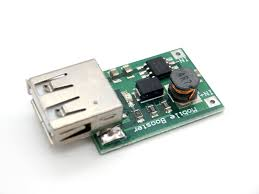
\includegraphics{boostconverter.jpeg}
     \caption{Boost Converter [2].}
     \label{fig:boostconverter}
\end{figure}

\subsection{Organization Tree}

Organization tree can be seen from the figure \ref{fig:organization tree}.

\begin{figure}
     \centering
     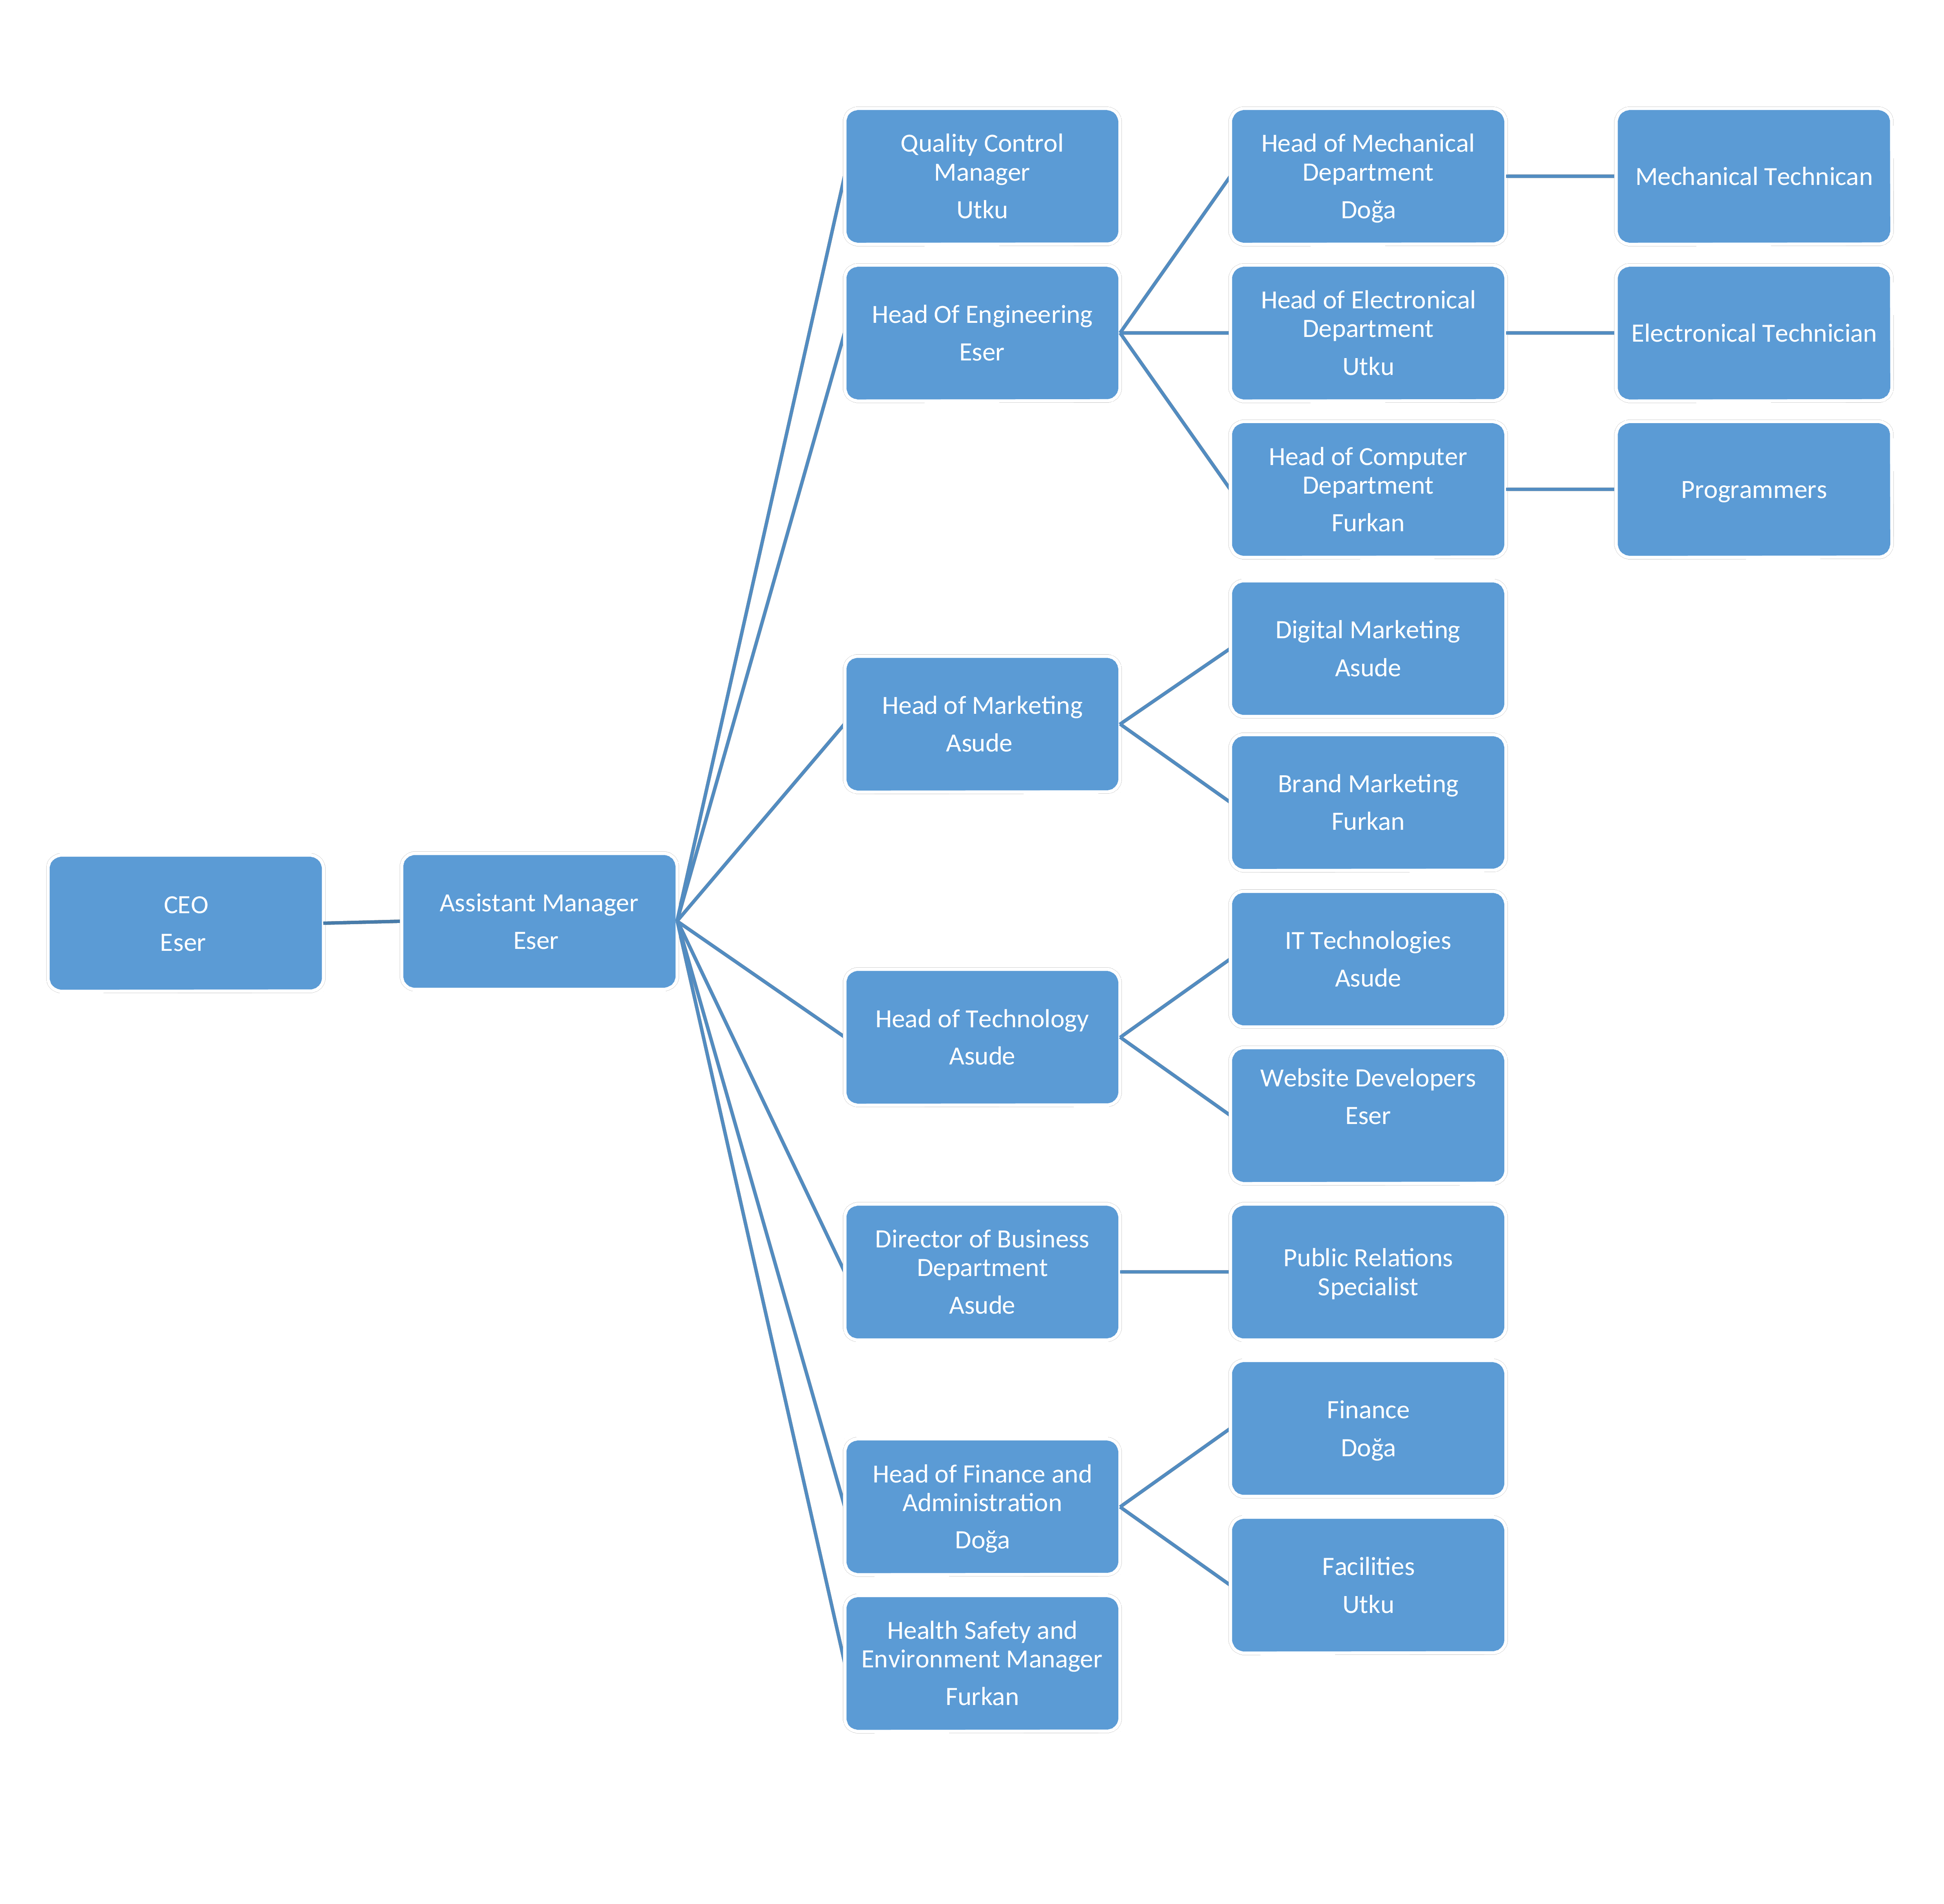
\includegraphics[width=16cm]{organizationtree.png}
     \caption{Organization Tree.}
     \label{fig:organization tree}
\end{figure}